\documentclass[12pt,a4paper]{article}
\usepackage[utf8]{inputenc}
\usepackage{amsmath}
\usepackage{amsfonts}
\usepackage{amssymb}
\usepackage{listings}
\usepackage{url}
\usepackage[bulgarian]{babel}
\usepackage{listings}
\usepackage{enumerate}
\usepackage{hyperref}
\usepackage{relsize}
\usepackage{graphicx}


\lstset{breaklines=true} 


\author{\textit{email: kalin@fmi.uni-sofia.bg}}
\title{\textsc{Задачи за задължителна самоподготовка} \\
по \\
Структури от данни и програмиране\\
\textit{Двоични дървета, стек, итератори}}




\begin{document}
\maketitle

 \underline{Упътване}:Решете задачите с рекурсия и след това преобразувайте решението в решение със стек.



\begin{enumerate}

	\item Да се дефинира функция за намиране на стойността на полинома на Ермит $Hn(x)$ (x е реална променлива, а n неотрицателна цяла променлива), дефиниран по следния начин:

	$H_0(x)=1$

	$H_1(x)=2x$

	$H_n(x)=2xH_{n-1}(x)+2(n-1)H_{n-2}(x), n>1$,

	за дадени $n$ и $x$ \underline{с използване на стек}.


	\item Нека е дадена абстрактна шахматна дъска с размери $n \times n$, $4 \le n \le 8$ и число $k$, $0 \le k \le n$. Казваме, че разположени на дъската  $k$ коня образуват ``валидна конфигурация'', ако никоя фигура не е поставена на поле, което се ``бие'' от друга фигура според съответните шахматни правила. 

	Да се дефинира клас \texttt{HorseConfig}, представящ ``конфигуратор'' на шахматни коне. Конструкторът на класа инициализира конфигуратора с числата $n$ и $k$. Класът позволява ``обхождането'' една по една на всички валидни конфигурации за дадените параметри, по подобие на \texttt{forward} итератор на структура от данни. Класът да притежава следните методи:

	\begin{itemize}
		\item \texttt{void HorseConfig::printCurrentConfig()}: Отпечатва текущо намерената конфигурация.
			Пример за отпечатана конфигурация с $n=5, k=2$:
			\begin{verbatim}
			_ _ _ _ _
			_ _ H _ _
			_ _ _ _ _
			_ _ _ _ H
			_ _ _ _ _
				
			\end{verbatim}		
		\item \texttt{void HorseConfig::findNextConfig()}: Намира следваща конфигурация.
		\item \texttt{bool HorseConfig::noMoreConfigs()}: Показва дали всички възможни конфигурации са вече изчерпани.
	\end{itemize}


	%\vspace{-70px}
	\begin{flushleft}
	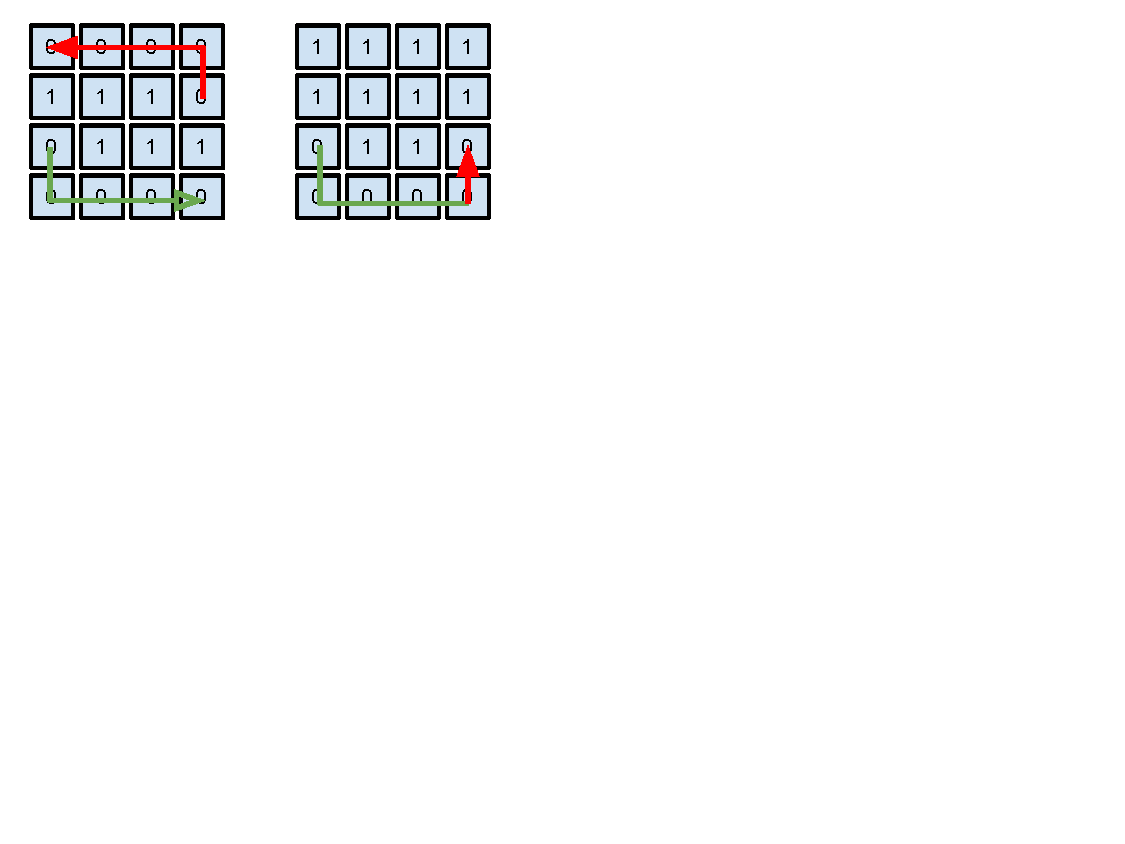
\includegraphics[width=15cm]{images/path1}
	\vspace{-250px}
	\relscale{0.8}
	\end{flushleft}
	Фигура 1a и 1б. Примерени лабиринти

	\item Нека е дадена квадратна матрица от цели числа $N \times N$, представяща ``лабиринт''. Елементи на матрицата със стойност $0$ смятаме за ``проходими'', а всички останали - за ``непроходими''. Път в лабиринта наричаме всяка последователност от проходими елементи на матрицата, които са съседни вертикално или хоризонтално, такава че (1) никой елемент от последователноста не е последван директно от предшественика си (забранено е ``връщането назад'') и (2) най-много един елемент на последователноста се среща в нея повече от веднъж (има най-много един ``цикъл'').

	Да се дефинира функция \texttt{bool downstairs (int sx, int sy, int tx, int ty)}, която проверява дали съществува път от елемента $(sx,sy)$ до елемента $(tx,ty)$, такъв, че всеки следващ елемент от пътя е или вдясно, или под предишния. Такъв път да наричаме ``низходящ''. 

	Пример: На фигура 1a такъв път съществува от елемента $(0,2)$ до елемента $(3,3)$, но не и от $(3,1)$ до $(0,0)$.

	Решението да е чрез използване на стек.

	\item Разработеният на лекции итератор на клас \texttt{BTree<T>} да бъде видоизменен така, че:

	\begin{enumerate}
		\item Да се промени обхождането от ЛКД на КДЛ и ЛДК.
		\item Да бъдат обхождани само листата на дървото, в нарастващ ред (за случаите на двоично-наредено дърво).
		\item Итераторът да може да се инициализира с предикат \texttt{bool pred (const T\&)} и обхождането на включва само тези елементи на дървото, които удовлетворяват предиката.

	\end{enumerate}





\end{enumerate}






\end{document}

